%%%%%%%%%%%%%%%%%%%%%%%%%%%%%%%%%%%%%%%%%
% Programming/Coding Assignment
% LaTeX Template
%
% This template has been downloaded from:
% http://www.latextemplates.com
%
% Original author:
% Ted Pavlic (http://www.tedpavlic.com)
%
% Note:
% The \lipsum[#] commands throughout this template generate dummy text
% to fill the template out. These commands should all be removed when 
% writing assignment content.
%
% This template uses a Perl script as an example snippet of code, most other
% languages are also usable. Configure them in the "CODE INCLUSION 
% CONFIGURATION" section.
%
%%%%%%%%%%%%%%%%%%%%%%%%%%%%%%%%%%%%%%%%%

%----------------------------------------------------------------------------------------
%	PACKAGES AND OTHER DOCUMENT CONFIGURATIONS
%----------------------------------------------------------------------------------------

%\documentclass{article}
\documentclass[12pt]{article}
\usepackage{fancyhdr} % Required for custom headers
\usepackage{lastpage} % Required to determine the last page for the footer
\usepackage{extramarks} % Required for headers and footers
\usepackage[usenames,dvipsnames]{color} % Required for custom colors
\usepackage{graphicx} % Required to insert images
\usepackage{subcaption}
\usepackage{listings} % Required for insertion of code
\usepackage{courier} % Required for the courier font
\usepackage{amsmath}
\usepackage{framed}

% Margins
\topmargin=-0.45in
\evensidemargin=0in
\oddsidemargin=0in
\textwidth=6.5in
\textheight=9.0in
\headsep=0.25in

\linespread{1.1} % Line spacing

% Set up the header and footer
\pagestyle{fancy}
\lhead{\hmwkAuthorName} % Top left header
\chead{\hmwkClass\ (\hmwkClassTime): \hmwkTitle} % Top center head
%\rhead{\firstxmark} % Top right header
\lfoot{\lastxmark} % Bottom left footer
\cfoot{} % Bottom center footer
\rfoot{Page\ \thepage\ of\ \protect\pageref{LastPage}} % Bottom right footer
\renewcommand\headrulewidth{0.4pt} % Size of the header rule
\renewcommand\footrulewidth{0.4pt} % Size of the footer rule

\setlength\parindent{0pt} % Removes all indentation from paragraphs

%----------------------------------------------------------------------------------------
%	CODE INCLUSION CONFIGURATION
%----------------------------------------------------------------------------------------

\definecolor{mygreen}{rgb}{0,0.6,0}
\definecolor{mygray}{rgb}{0.5,0.5,0.5}
\definecolor{mymauve}{rgb}{0.58,0,0.82}

\lstset{ %
  backgroundcolor=\color{white},   % choose the background color
  basicstyle=\footnotesize,        % size of fonts used for the code
  breaklines=true,                 % automatic line breaking only at whitespace
  captionpos=b,                    % sets the caption-position to bottom
  commentstyle=\color{mygreen},    % comment style
  escapeinside={\%*}{*)},          % if you want to add LaTeX within your code
  keywordstyle=\color{blue},       % keyword style
  stringstyle=\color{mymauve},     % string literal style
}

%----------------------------------------------------------------------------------------
%	DOCUMENT STRUCTURE COMMANDS
%	Skip this unless you know what you're doing
%----------------------------------------------------------------------------------------

% Header and footer for when a page split occurs within a problem environment
\newcommand{\enterProblemHeader}[1]{
%\nobreak\extramarks{#1}{#1 continued on next page\ldots}\nobreak
%\nobreak\extramarks{#1 (continued)}{#1 continued on next page\ldots}\nobreak
}

% Header and footer for when a page split occurs between problem environments
\newcommand{\exitProblemHeader}[1]{
%\nobreak\extramarks{#1 (continued)}{#1 continued on next page\ldots}\nobreak
%\nobreak\extramarks{#1}{}\nobreak
}

\setcounter{secnumdepth}{0} % Removes default section numbers
\newcounter{homeworkProblemCounter} % Creates a counter to keep track of the number of problems
\setcounter{homeworkProblemCounter}{0}

\newcommand{\homeworkProblemName}{}
\newenvironment{homeworkProblem}[1][Problem \arabic{homeworkProblemCounter}]{ % Makes a new environment called homeworkProblem which takes 1 argument (custom name) but the default is "Problem #"
\stepcounter{homeworkProblemCounter} % Increase counter for number of problems
\renewcommand{\homeworkProblemName}{#1} % Assign \homeworkProblemName the name of the problem
\section{\homeworkProblemName} % Make a section in the document with the custom problem count
\enterProblemHeader{\homeworkProblemName} % Header and footer within the environment
}{
\exitProblemHeader{\homeworkProblemName} % Header and footer after the environment
}

\newcommand{\problemAnswer}[1]{ % Defines the problem answer command with the content as the only argument
\noindent\framebox[\columnwidth][c]{\begin{minipage}{0.98\columnwidth}#1\end{minipage}} % Makes the box around the problem answer and puts the content inside
}

\newcommand{\homeworkSectionName}{}
\newenvironment{homeworkSection}[1]{ % New environment for sections within homework problems, takes 1 argument - the name of the section
\renewcommand{\homeworkSectionName}{#1} % Assign \homeworkSectionName to the name of the section from the environment argument
\subsection{\homeworkSectionName} % Make a subsection with the custom name of the subsection
\enterProblemHeader{\homeworkProblemName\ [\homeworkSectionName]} % Header and footer within the environment
}{
\enterProblemHeader{\homeworkProblemName} % Header and footer after the environment
}

%----------------------------------------------------------------------------------------
%	NAME AND CLASS SECTION
%----------------------------------------------------------------------------------------

\newcommand{\hmwkTitle}{Assignment 1} % Assignment title
\newcommand{\hmwkDueDate}{Friday, Feb 8, 2018} % Due date
\newcommand{\hmwkClass}{CSC412} % Course/class
\newcommand{\hmwkClassTime}{LEC 0101} % Class/lecture time
\newcommand{\hmwkAuthorName}{Zhongtian Ouyang} % Your name
\newcommand{\hmwkAuthorID}{1002341012} % Your name

%----------------------------------------------------------------------------------------
%	TITLE PAGE
%----------------------------------------------------------------------------------------

\title{
\vspace{2in}
\textmd{\textbf{\hmwkClass:\ \hmwkTitle}}\\
\normalsize\vspace{0.1in}\small{Due\ on\ \hmwkDueDate}\\
\vspace{0.1in}
\vspace{3in}
}

\author{\textbf{\hmwkAuthorName}\\ \textbf{\hmwkAuthorID}}

\date{(collaborate with Yihao Ni)} % Insert date here if you want it to appear below your name

%----------------------------------------------------------------------------------------\
\begin{document}

\maketitle
\clearpage

%----------------------------------------------------------------------------------------
%	Common Tools
%----------------------------------------------------------------------------------------
%\begin{framed}
%\begin{lstlisting}[language=matlab]
%\end{lstlisting}
%\end{framed}

% \begin{bmatrix}
%0.5 & 0.6 \\ 
%0.7 & 0.8
%\end{bmatrix}

%\begin{figure}[h!]
%\centering
%\includegraphics[width=0.6\linewidth]{q10a.png}
%\label{fig:q10a}
%\end{figure}\\

%\begin{figure*}[!ht]
%\begin{subfigure}{.5\textwidth}
% \centering
%  \includegraphics[width=.5\linewidth]{p4_1.JPG}
%  \caption{Full set}
%  \label{fig:sfig1}
%\end{subfigure}
%\begin{subfigure}{.5\textwidth}
% \centering
%  \includegraphics[width=.5\linewidth]{P4_2.JPG}
%  \caption{Two each}
%  \label{fig:sfig2}
%\end{subfigure}%
%\caption{Part4 (a)}
%\label{fig:p4a}
%\end{figure*}

%\sum_{n=1}^{\infty} 2^{-n} = 1
%\prod_{i=a}^{b} f(i)

%\begin{equation}
%\begin{split}
%1+2+3+4+8x+7 & =1+2+3+4+4x+35 \\
%& \Rightarrow x=7
%\end{split}
%\end{equation}
%----------------------------------------------------------------------------------------
%	PROBLEM 1
%----------------------------------------------------------------------------------------

% To have just one problem per page, simply put a \clearpage after each problem
\begin{homeworkProblem}
The proves are for discrete variables. For continuous variables, just change sum to integration and everything else should be almost the same.
(a)\\
For two independent variables X, Y:\\
$P(X \cap Y) = P(X)P(Y)$\\
$E[XY] = \sum_x\sum_y xyP(x, y) = \sum_x\sum_y xyP(x)P(y) =  (\sum_x xP(x))(\sum_y yP(y)) = E[X]E[Y]$
$Cov(X,Y) = E[XY] - E[X]E[Y] = E[X]E[Y] - E[X]E[Y] = 0$\\

(b)\\
\begin{equation}
\begin{split}
E[X+\alpha Y] &= \sum_x\sum_y (x+\alpha y)P(x, y) \\
&= \sum_x\sum_y xP(x, y)  +  \sum_x\sum_y \alpha yP(x, y) \\
&= \sum_x xP(x) +\alpha \sum_y yP(y) \\
&= E[x] + \alpha E[y]
\end{split}
\end{equation}

\begin{equation}
\begin{split}
V[X+\alpha Y] &= E[((X+\alpha Y) - E[X+\alpha Y])^2] \\
&= E[((X - \mu_x) + (\alpha Y - \alpha \mu_y))^2] \\
&= E[((X - \mu_x) + \alpha(Y - \mu_y))^2] \\
&= E[(X - \mu_x)^2 + 2(X - \mu_x)\alpha(Y - \mu_y) + \alpha^2(Y - \mu_y)^2]\\
&= V[X] + 2\alpha Cov(X,Y) + \alpha^2V[Y]\\
&= V[X] + \alpha^2V[Y]
\end{split}
\end{equation}

\end{homeworkProblem}
\clearpage
%----------------------------------------------------------------------------------------
%	PROBLEM 2
%----------------------------------------------------------------------------------------

\begin{homeworkProblem}
(a)\\
For continuous random variables, its pdf at some value can be greater than 1 as long as the area under the curve sums to 1.\\

(b)\\
$$f(x|\mu = 0, \sigma^2 = \frac{1}{100}) 
= \frac{1}{\sqrt{2\pi \frac{1}{100}}}e^{-\frac{(x-0)^2}{2\frac{1}{100}}} 
= \frac{1}{\sqrt{\frac{\pi}{50}}}e^{-50x^2} $$

(c)\\
$$f(0|\mu = 0, \sigma^2 = \frac{1}{100}) = \frac{1}{\sqrt{\frac{\pi}{50}}}e^{-50*0^2} = 3.9894$$

(d)\\
The probability that X=0 is 0.\\

\end{homeworkProblem}
\clearpage
%----------------------------------------------------------------------------------------
%	PROBLEM 3
%----------------------------------------------------------------------------------------

\begin{homeworkProblem}
(a)\\
$$r = x^Ty = \sum_{i=1}^{m}x_i * y_i$$
$$\frac{\partial r}{\partial x_i} = y_i$$
$$\frac{\partial x^Ty}{\partial x} = y$$

(b)\\
$$r = x^Tx = \sum_{i=1}^{m}x_i * x_i =  \sum_{i=1}^{m}x_i^2$$
$$\frac{\partial r}{\partial x_i} = 2*x_i$$
$$\frac{\partial x^Tx}{\partial x} = 2x$$

(c)\\
$$r = x^TA,\ r_i = \sum_{j=1}^{m} x_j a_{ji}$$
$$\frac{\partial r}{\partial x} = J = 
\begin{bmatrix}
\frac{\partial r_1}{\partial x_1} & ... & \frac{\partial r_1}{\partial x_m}\\ 
 & \vdots & \\
\frac{\partial r_m}{\partial x_1} & ... & \frac{\partial r_m}{\partial x_m}
\end{bmatrix}
= 
\begin{bmatrix}
a_{11} & ... & a_{m1}\\ 
 & \vdots & \\
a_{1m}  & ... & a_{mm}
\end{bmatrix}
$$
$$\frac{\partial x^TA}{\partial x} = J = A^T$$

(d)\\
let $r = x^TA$, $y = x$\\
$z = x^TAx = ry = (r_1x_1 + ... + r_mx_m) = (a_{11}x_1 + ... + a_{m1}x_m)x_1 + ... +  (a_{1m}x_1 + ... + a_{mm}x_m)x_m$:\\
$$\frac{\partial z}{\partial x} = \frac{\partial z}{\partial r} \frac{\partial r}{\partial x} +  \frac{\partial z}{\partial y}\frac{\partial y}{\partial x}  = x^TA^T + r = x^TA^T + x^TA = x^T(A + A^T)$$

\end{homeworkProblem}
\clearpage
%----------------------------------------------------------------------------------------
%	PROBLEM 4
%----------------------------------------------------------------------------------------

\begin{homeworkProblem}

(a)\\
$Y = X\beta + \epsilon$ where $\epsilon$ is the difference between $Y$ and $X\beta$, the noise from variance. $E[\epsilon|X] = 0$\\
\begin{equation}
\begin{split}
\hat\beta & =(X^TX)^{-1}X^TY\\
& = (X^TX)^{-1}X^T(X\beta + \epsilon)\\
& = \beta + (X^TX)^{-1}X^T \epsilon\\
\end{split}
\end{equation}
$$E[\hat\beta] = E[\beta + (X^TX)^{-1}X^T \epsilon] = \beta + (X^TX)^{-1}E[X^T \epsilon] = \beta$$
\begin{equation}
\begin{split}
V[\hat\beta] & = E[(\hat\beta - \beta)(\hat\beta - \beta)^T]\\
& = E[((X^TX)^{-1}X^T \epsilon)((X^TX)^{-1}X^T \epsilon)^T]\\
& = E[(X^TX)^{-1}X^T \epsilon\epsilon^TX(X^TX)^{-1}] \\
& = (X^TX)^{-1}X^T E[\epsilon\epsilon^T]X(X^TX)^{-1}\\
& =  (X^TX)^{-1}X^T\sigma^2IX(X^TX)^{-1}\\
& = \sigma^2(X^TX)^{-1}X^TX(X^TX)^{-1}\\
& = \sigma^2(X^TX)^{-1}
\end{split}
\end{equation}

(b)\\
Likelihood function for $\beta$ is:\\
\begin{equation}
\begin{split}
L(Y|X, \beta, \sigma^2I)& = \prod_{i = 1}^{n} \frac{1}{det(2\pi\sum)^{\frac{1}{2}}}e^{-\frac{1}{2}(y_i-\mu_i)^T\sum^{-1}(y_i-\mu_i)}\\
& = \prod_{i = 1}^{n} \frac{1}{det(2\pi\sigma^2I)^{\frac{1}{2}}}e^{-\frac{1}{2}(y_i-x_i\beta)^T(\sigma^2I)^{-1}(y_i-x_i\beta)}\\
& = \prod_{i = 1}^{n} \frac{1}{det(2\pi\sigma^2I)^{\frac{1}{2}}}e^{-\frac{1}{2}\sigma^{-2}I(y_i-x_i\beta)^T(y_i-x_i\beta)}\\
&=\frac{1}{det(2\pi\sigma^2I)^{\frac{n}{2}}}e^{\sum_{i=1}^n -\frac{1}{2}\sigma^{-2}I(y_i-x_i\beta)^T(y_i-x_i\beta)}\\
&= \frac{1}{det(2\pi\sigma^2I)^{\frac{n}{2}}}e^{-\frac{1}{2}\sigma^{-2}I\sum_{i=1}^n(y_i-x_i\beta)^T(y_i-x_i\beta)}\\
&= \frac{1}{det(2\pi\sigma^2I)^{\frac{n}{2}}}e^{-\frac{1}{2}\sigma^{-2}I (Y-X\beta)^T(Y-X\beta)}\\
\end{split}
\end{equation}
When we find an $\beta$ that minimize $\sum_{i=1}^n(y_i-x_i\beta)^2$, since $\sum_{i=1}^n(y_i-x_i\beta)^2 = (Y-X\beta)^T(Y-X\beta)$, such $\beta$ also minimize $(Y-X\beta)^T(Y-X\beta)$.
Therefore, such $\beta$ would maximize the term
$e^{-\frac{1}{2}\sigma^{-2}I(Y-X\beta)^T(Y-X\beta)}$ and maxmize the likelihood function.\\
An $\beta$ that maxmize the likelihood function would also be minimizing the square error\\
Without even using a log likelihood trick, we can conclude that minimizing square error is equivalent to maximizin the likelihood.\\

(c)\\
\begin{equation}
\begin{split}
\sum_{i=1}^n(y_i-x_i\beta)^2 &= (Y-X\beta)^T(Y-X\beta)\\
& = Y^TY - Y^TX\beta - \beta^TX^TY + \beta^TX^TX\beta\\
& = Y^TY - 2\beta^TX^TY + \beta^TX^TX\beta
\end{split}
\end{equation}
\end{homeworkProblem}

(d)\\
\begin{equation}
\begin{split}
\frac{\partial}{\partial \beta}( Y^TY - 2\beta^TX^TY + \beta^TX^TX\beta)
& = \frac{\partial  Y^TY}{\partial \beta} - \frac{\partial 2\beta^TX^TY}{\partial \beta} +  \frac{\partial  \beta^TX^TX\beta}{\partial \beta}\\
& = 0 - 2Y^TX + \beta^T(X^TX + (X^TX)^T)\\
& = 0 - 2Y^TX + 2\beta^T(X^TX)\\
\end{split}
\end{equation}
Since both $2Y^TX$ and $2\beta^T(X^TX)$ vectors, $0 - 2Y^TX + 2\beta^T(X^TX)$ and $0 - 2X^TY + 2(X^TX)\beta$ are the same except one is row vector, the other is column vector. To find $\beta=\hat{\beta}$ minimize the error, we set derivative equals to zero\\
$$- 2X^TY + 2(X^TX)\hat{\beta} = 0$$
$$X^TY = (X^TX)\hat{\beta}$$
$$\hat{\beta} = (X^TX)^{-1}X^TY$$
\clearpage
%----------------------------------------------------------------------------------------
%	PROBLEM 5
%----------------------------------------------------------------------------------------

\begin{homeworkProblem}
(a)\\
$$argmax_{\hat{\beta}}\frac{P(y|\beta = \hat{\beta})P(\beta = \hat{\beta})}{P(y)} 
= argmax_{\hat{\beta}}P(y|\beta = \hat{\beta})P(\beta = \hat{\beta}) 
= argmax_{\hat{\beta}}lnP(y|\beta = \hat{\beta})+ lnP(\beta = \hat{\beta})$$
$$P(y|\beta = \hat{\beta}) =\prod_{i = 1}^{n} \frac{1}{det(2\pi\sum)^{\frac{1}{2}}}e^{-\frac{1}{2}(y_i-\mu_i)^T\sum^{-1}(y_i-\mu_i)}$$
\begin{equation}
\begin{split}
ln P(y|\beta = \hat{\beta}) 
&= -\frac{n^2}{2}ln(2\pi) - \frac{n}{2}ln(det(\sum)) - \frac{1}{2}\sum_{i=1}^{n}(y_i-\mu_i)^T(\sum)^{-1}(y_i-\mu_i)\\
&= -\frac{n^2}{2}ln(2\pi) - \frac{n}{2}ln(det(\sigma^2I)) - \frac{1}{2}\sum_{i=1}^{n}(y_i-x_i\beta)^T(\sigma^2I))^{-1}(y_i-x_i\beta)\\
& = -\frac{n^2}{2}ln(2\pi) - \frac{n}{2}ln(\sigma^{2n}det(I)) -  \frac{1}{2}\sum_{i=1}^{n}(y_i-x_i\beta)^T\sigma^{-2}I(y_i-x_i\beta)\\
& = -\frac{n^2}{2}ln(2\pi) - \frac{n^2}{2}ln(\sigma^2) -  \frac{1}{2}\sigma^{-2}I(Y-X\beta)^T(Y-X\beta)\\
\end{split}
\end{equation}

$$
P(\beta = \hat{\beta}) 
= \frac{1}{det(2\pi\sum)^{\frac{1}{2}}}e^{-\frac{1}{2}(\beta-0)^T (\sum)^{-1} (\beta-0)}\\
= \frac{1}{2\pi^{\frac{m}{2}}det(\sum)^{\frac{1}{2}}}e^{-\frac{1}{2}\beta^T (\sum)^{-1} \beta}$$
\begin{equation}
\begin{split}
lnP(\beta = \hat{\beta})  
&= -\frac{m}{2}ln(det(2\pi))-\frac{1}{2}ln(det(\sum))-\frac{1}{2}\beta^T(\sum)^{-1}\beta\\
&= -\frac{m}{2}ln(det(2\pi))-\frac{1}{2}ln(det(\tau^2I)) - \frac{1}{2}\beta^T(\tau^2I)^{-1}\beta\\
&=-\frac{m}{2}ln(det(2\pi)) - \frac{m}{2}ln(\tau^2) - \frac{1}{2}\tau^{-2}I\beta^T\beta
\end{split}
\end{equation}

$$F = lnP(y|\beta = \hat{\beta})+ lnP(\beta = \hat{\beta})$$
\begin{equation}
\begin{split}
\frac{\partial}{\partial\beta}F 
&= 0 + 0 + \frac{\partial}{\partial\beta}(-\frac{1}{2}\sigma^{-2}I(Y-X\beta)^T(Y-X\beta)) + 0 + 0 + \frac{\partial}{\partial\beta}(- \frac{1}{2}\tau^{-2}I\beta^T\beta)\\
&=-\frac{1}{2}\sigma^{-2}I(- 2X^TY + 2(X^TX)\beta) - \frac{1}{2}\tau^{-2}I(2\beta)\\
& = -\frac{1}{2}\sigma^{-2}I(- 2X^TY + 2(X^TX)\beta) - \tau^{-2}I\beta\\
\end{split}
\end{equation}

let $\beta = \hat{\beta}$ such that $\frac{\partial}{\partial\beta}F = 0$
\begin{equation}
\begin{split}
0 & = -\frac{1}{2}\sigma^{-2}I(- 2X^TY + 2(X^TX)\hat{\beta}) - \tau^{-2}I\hat{\beta}\\
0 & = \sigma^{-2}IX^TY - \sigma^{-2}I(X^TX)\hat{\beta} - \tau^{-2}I\hat{\beta}\\
(\sigma^{-2}I(X^TX) + \tau^{-2}I)\hat{\beta}&=\sigma^{-2}IX^TY\\
\hat{\beta} &=  (\sigma^{-2}I(X^TX) + \tau^{-2}I)^{-1}\sigma^{-2}IX^TY\\
\hat{\beta} &= (\sigma^{2}I^{-1}\sigma^{-2}I(X^TX) + \sigma^{2}I^{-1}\tau^{-2}I)^{-1}X^TY\\
\hat{\beta} &= (X^TX + \frac{\sigma^{2}}{\tau^{2}}I)^{-1}X^TY\\
\hat{\beta}_{MAP} &= (X^TX + \lambda I)^{-1}X^TY
\end{split}
\end{equation}
\clearpage
(b)\\
Modified X and Y:
$$
\bar X = 
 \begin{bmatrix}
x_{11} & ... & x_{1m}\\
\vdots & & \vdots\\
x_{n1}& ... & x_{nm}\\
\sqrt\lambda & ... & 0\\
\vdots & \ddots & \vdots\\
0 & ... & \sqrt\lambda\\
\end{bmatrix}
,\ \ \bar Y = 
\begin{bmatrix}
y_1\\
\vdots\\
y_n\\
0\\
\vdots\\
0\\
\end{bmatrix}
$$
\begin{equation}
\begin{split}
\bar X^T\bar X &= 
 \begin{bmatrix}
x_{11} & ... & x_{n1}& \sqrt\lambda& ... & 0 \\
\vdots&  & \vdots& \vdots& \ddots & \vdots \\
x_{1m} & ... & x_{nm}& 0& ... & \sqrt\lambda \\
\end{bmatrix}
 \begin{bmatrix}
x_{11} & ... & x_{1m}\\
\vdots & & \vdots\\
x_{n1}& ... & x_{nm}\\
\sqrt\lambda & ... & 0\\
\vdots & \ddots & \vdots\\
0 & ... & \sqrt\lambda\\
\end{bmatrix}\\
&=
\begin{bmatrix}
\sum_{i=1}^{n}x_{i1}^2+\lambda & \sum_{i=1}^{n}x_{i2}x_{i1} & ... & \sum_{i=1}^{n}x_{im}x_{i1}\\
\sum_{i=1}^{n}x_{i1}x_{i2} & \sum_{i=1}^{n}x_{i2}^2+\lambda & ... & \sum_{i=1}^{n}x_{im}x_{i2}\\
\vdots&\vdots &\ddots&\vdots\\
\sum_{i=1}^{n}x_{i1}x_{im} & \sum_{i=1}^{n}x_{i2}x_{im} & ... & \sum_{i=1}^{n}x_{im}^2 + \lambda \\
\end{bmatrix}
\end{split}
\end{equation}

\begin{equation}
\begin{split}
X^TX + \lambda I&= 
 \begin{bmatrix}
x_{11} & ... & x_{n1} \\
\vdots&  & \vdots\\
x_{1m} & ... & x_{nm}\\
\end{bmatrix}
 \begin{bmatrix}
x_{11} & ... & x_{1m}\\
\vdots & & \vdots\\
x_{n1}& ... & x_{nm}\\
\end{bmatrix}
+ 
\begin{bmatrix}
\lambda & & 0\\
 & \ddots & \\
0& ... & \lambda\\
\end{bmatrix}\\
&=
\begin{bmatrix}
\sum_{i=1}^{n}x_{i1}^2& \sum_{i=1}^{n}x_{i2}x_{i1} & ... & \sum_{i=1}^{n}x_{im}x_{i1}\\
\sum_{i=1}^{n}x_{i1}x_{i2} & \sum_{i=1}^{n}x_{i2}^2 & ... & \sum_{i=1}^{n}x_{im}x_{i2}\\
\vdots&\vdots &\ddots&\vdots\\
\sum_{i=1}^{n}x_{i1}x_{im} & \sum_{i=1}^{n}x_{i2}x_{im} & ... & \sum_{i=1}^{n}x_{im}^2\\
\end{bmatrix}
+
\begin{bmatrix}
\lambda & & 0\\
 & \ddots & \\
0& ... & \lambda\\
\end{bmatrix}\\
&= 
\begin{bmatrix}
\sum_{i=1}^{n}x_{i1}^2+\lambda & \sum_{i=1}^{n}x_{i2}x_{i1} & ... & \sum_{i=1}^{n}x_{im}x_{i1}\\
\sum_{i=1}^{n}x_{i1}x_{i2} & \sum_{i=1}^{n}x_{i2}^2+\lambda & ... & \sum_{i=1}^{n}x_{im}x_{i2}\\
\vdots&\vdots &\ddots&\vdots\\
\sum_{i=1}^{n}x_{i1}x_{im} & \sum_{i=1}^{n}x_{i2}x_{im} & ... & \sum_{i=1}^{n}x_{im}^2 + \lambda \\
\end{bmatrix}
\end{split}
\end{equation}
For $\bar X^T \bar Y$, since the last m columns of $\bar X^T$ are the added rows of $\bar X$ and last m rows of $\bar Y$ are the added value 0, $\bar X^T \bar Y = X^TY$\\
Therefore, the following is true:
$$(\bar X^T \bar X)^{-1}\bar X^T \bar Y = (X^TX + \lambda I)^{-1}X^TY$$
This shows that ridge regression with $X$ and $Y$ is equivalent to computing maximum likelihood estimate of $\beta$ using the modified $\bar X$ and $\bar Y$\\

\end{homeworkProblem}
\clearpage
%----------------------------------------------------------------------------------------
%	PROBLEM 6
%----------------------------------------------------------------------------------------
\begin{homeworkProblem}
1. \\
\begin{equation}
\begin{split}
distance\ of\ x\ from\ origin& = \sqrt{(x_1 - 0)^2 + (x_2 - 0)^2 + ... + (x_D - 0)^2}\\
& = \sqrt{x_1^2 + x_2^2 + ... + x_D^2}\\
& = \sqrt{x^Tx}
\end{split}
\end{equation}

2.\\
From the histogram below, we can see that most samples will be near the origin.
\begin{figure}[h!]
\centering
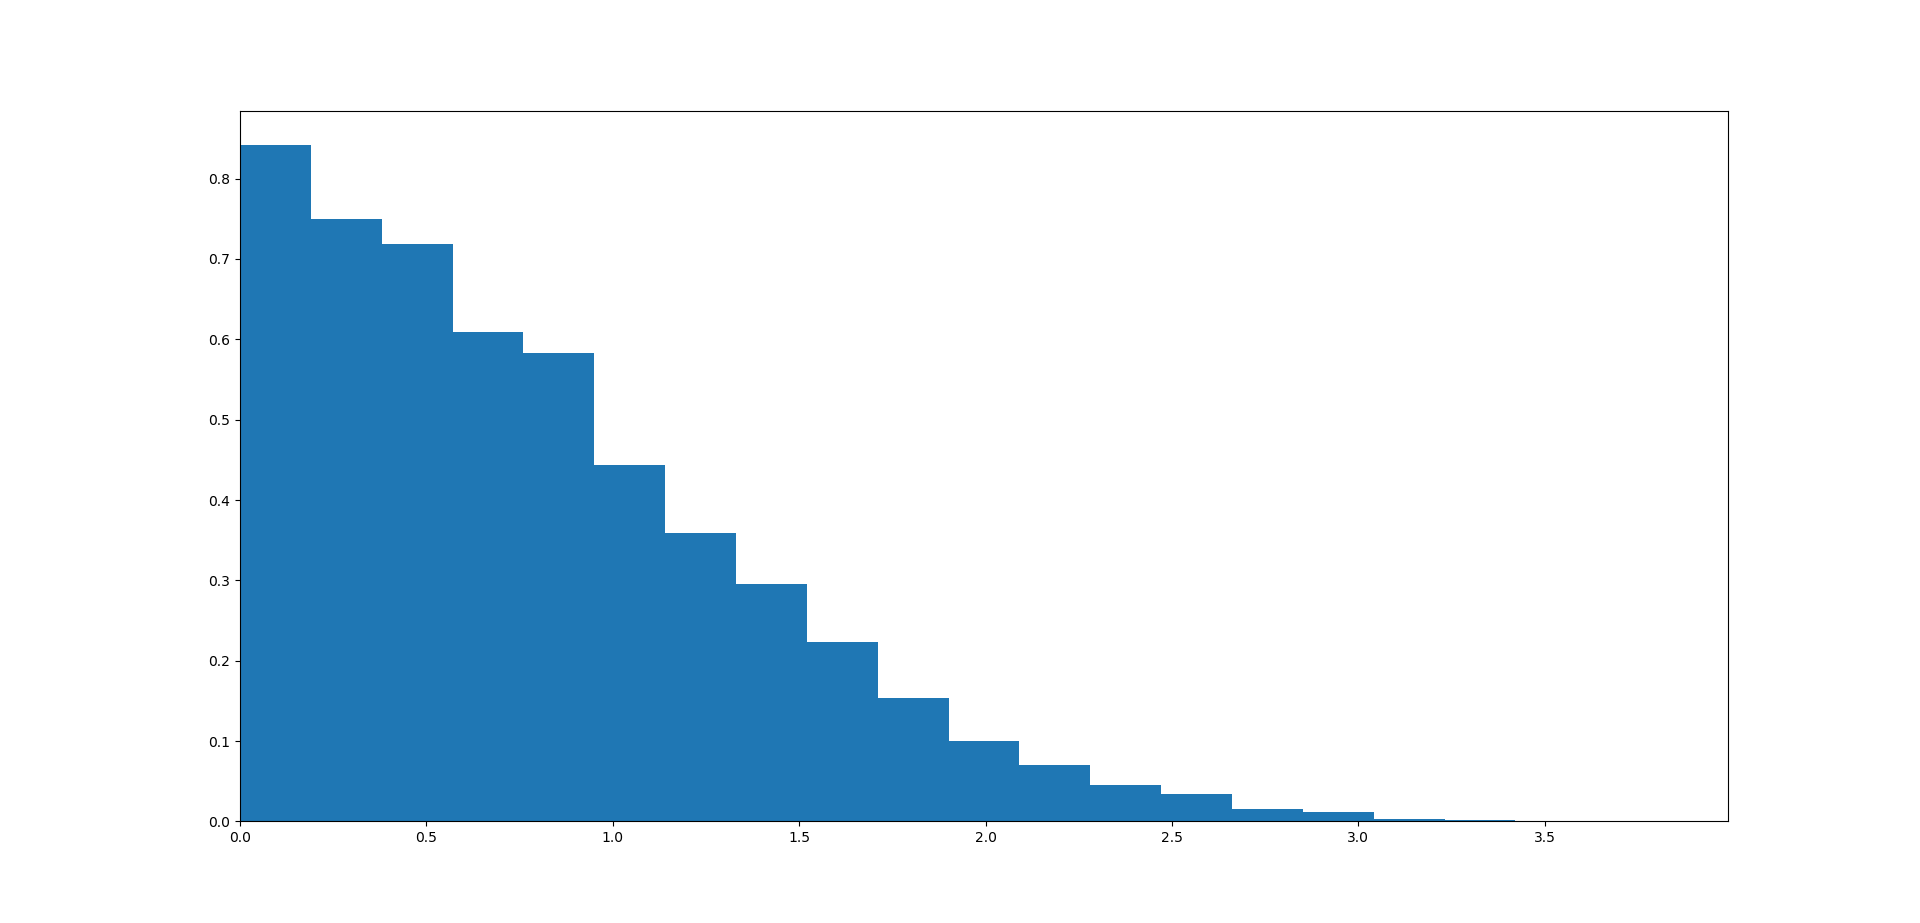
\includegraphics[width=0.8\linewidth]{Q2.png}
\end{figure}

3.\\
From the histograms in Figure 1 for different dimensions, we can observe that as the dimensionality of the Gaussian increases, the expected distance of the samples from the Gaussian's mean increase, shift away from 0.
\begin{figure*}[!ht]
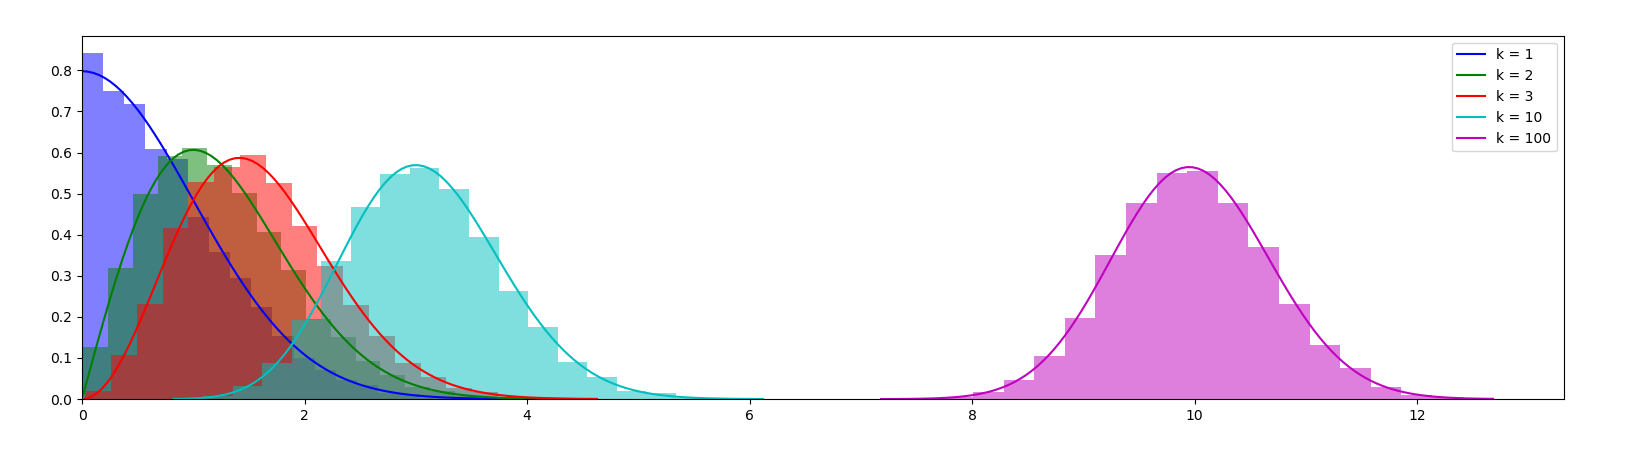
\includegraphics[width=1\linewidth]{Q3&4.png}
\caption{Question 3 \& 4}
\end{figure*}

4.\\
The lines in Figure 1 are the pdfs of the chi distribution with k = \{1,2,3,10,100\}\\

5.\\
$(x_a - x_b) \sim N(0_D, 2I_D)$\\
Because of euclidean distance and standard deviation is $\sqrt{2}$ of the previous. $Y = \sqrt{2}X$, $g^{-1}(Y) = (1/\sqrt{2}) Y$, $f_y(Y) = (1/\sqrt{2})f_x((1/\sqrt{2}) Y)$\\
Again, as the dimesionality increases, the distance between samples from a Gaussian increases.The mean shifts from 0 by about $\sqrt 2$ times of the previous question.
\begin{figure*}[!ht]
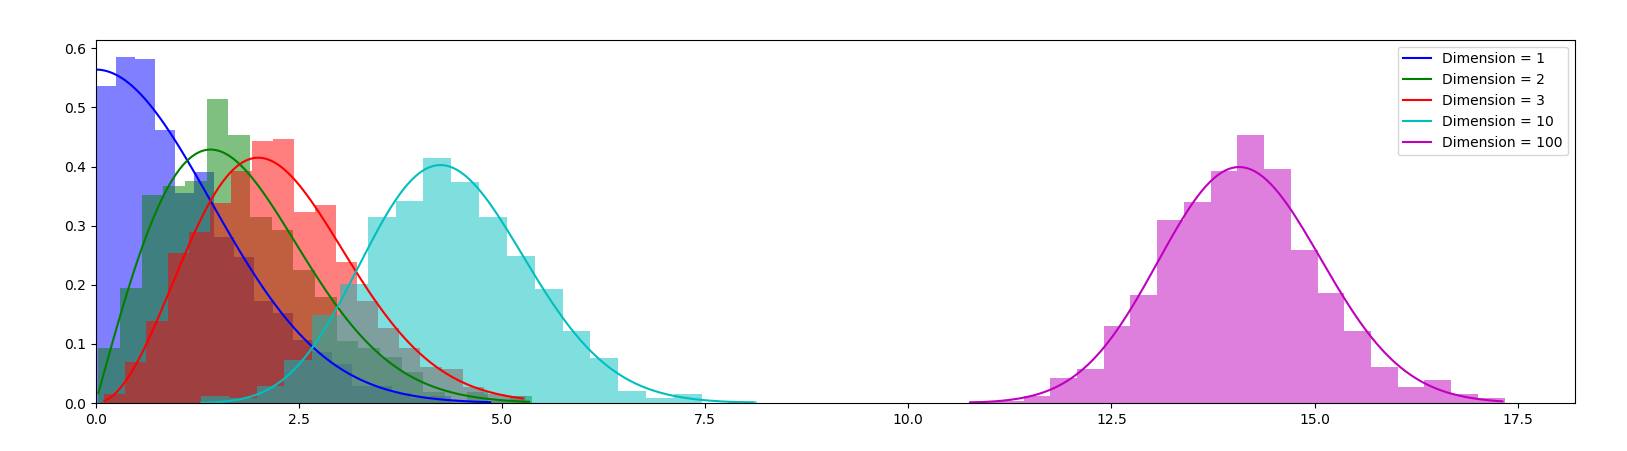
\includegraphics[width=1\linewidth]{Q5.png}
\caption{Question5}
\end{figure*}
\clearpage
6.\\
The log-likelihood increases as $\alpha$ approaching 0.5, reach the maximum, and then decrease as $\alpha$ approaching 1. The shape is identical for all dimensions. However, as the dimension increases, the overall value of log-likelihood decreases by a large amount. A higher log-likelihood for the interplolated points is not necessrily better. It is not a good idea to linearly interpolate between samples from a high dimensional Gaussian

7.\\
The log-likelihood is mostly flat for $\alpha \in [0,1]$. Polar interpolation is more suitable because the interpolates it provides are uniform and contain same level of information for high dimensional Gaussians.
\begin{figure*}[!ht]
\begin{subfigure}{0.4\textwidth}
 \centering
  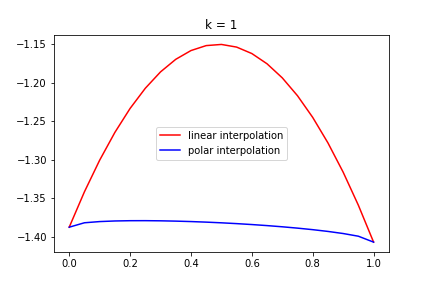
\includegraphics[width=1.1\linewidth]{Q6_1.png}
\end{subfigure}
\begin{subfigure}{0.4\textwidth}
 \centering
  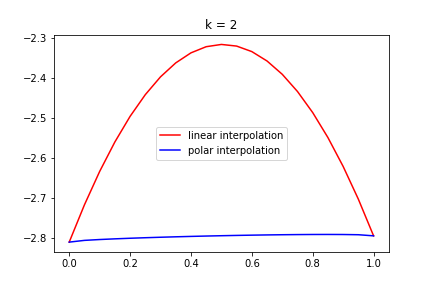
\includegraphics[width=1.1\linewidth]{Q6_2.png}
\end{subfigure}
\begin{subfigure}{0.4\textwidth}
 \centering
  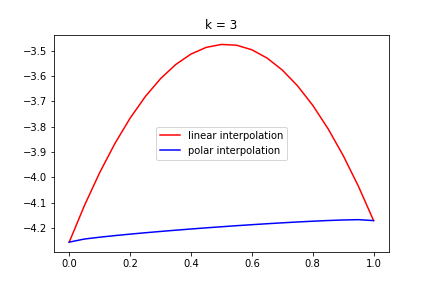
\includegraphics[width=1.1\linewidth]{Q6_3.png}
\end{subfigure}
\begin{subfigure}{0.4\textwidth}
 \centering
  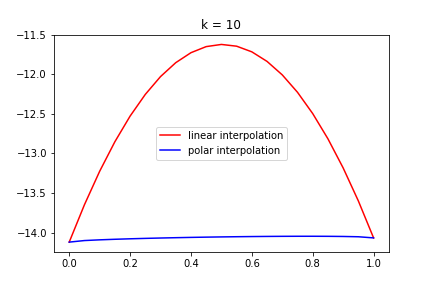
\includegraphics[width=1.1\linewidth]{Q6_10.png}
\end{subfigure}
\begin{subfigure}{0.4\textwidth}
 \centering
  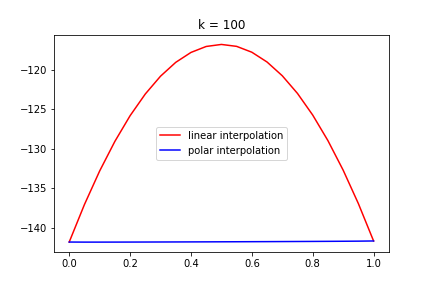
\includegraphics[width=1.1\linewidth]{Q6_100.png}
\end{subfigure}
\caption{Q6 \& 7}
\end{figure*}

\end{homeworkProblem}
%----------------------------------------------------------------------------------------

\end{document}
